\newcommand*{\tv}{\mathrm t}  % transverse
\newcommand*{\lt}{\mathrm l}  % longitudinal
\newcommand*{\Db}{\mathrm D}
\newcommand*{\Fm}{\mathrm F}

\chapter{Bose统计和Fermi统计}

不同于理想气体,实际气体不满足非简并条件,$\e\alpha\not\gg 1$,服从Bose分布和Fermi分布:
\begin{equation}
	a_i=\frac{\omega_i}{\e{\alpha+\beta\varepsilon_i}\pm 1},
\end{equation}
约定
$\pm$号的($+$)对应Fermi分布,($-$)对应Bose分布。
$\mp$号反之。

\begin{definition}{巨配分函数}{grand partition function}
	定义巨配分函数(grand partition function)的对数
	\begin{equation}
		\ln\Xi:=\pm\sum_i\omega_i\ln(1\pm\e{-\alpha-\beta\varepsilon_i}),
	\end{equation}
\end{definition}

\begin{corollary}
	根据巨配分函数可导出粒子数、内能、状态方程和熵等宏观量:
	\begin{subequations}
		\begin{align}
			N&=-\pv{\ln\Xi}\alpha,\\
			U&=-\pv{\ln\Xi}\beta,\\
			Y_k&=-\frac1\beta\pv{\ln\Xi}{y_k},\\
			S&=\kB(\ln\Xi+\alpha N+\beta U),\\
			\mu&=-\alpha\kB T.
		\end{align}
	\end{subequations}
\end{corollary}

\begin{proof}
	粒子数
	\[
		N=\sum_i a_i=\sum_i\frac{\omega_i}{\e{\alpha+\beta\varepsilon_i}\pm 1}=\mp\sum_i\omega_i\pp\alpha{\ln(1\pm\e{-\alpha-\beta\varepsilon_i})}=-\pv{\ln\Xi}\alpha,
	\]
	内能
	\[
		U=\sum_i a_i\varepsilon_i=\sum_i\frac{\omega_i\varepsilon_i}{\e{\alpha+\beta\varepsilon_i}\pm 1}=\mp\sum_i\omega_i\pp\beta{\ln(1\pm\e{-\alpha-\beta\varepsilon_i})}=-\pv{\ln\Xi}\beta,
	\]
	状态方程
	\[
		Y_k=-\sum_i a_i\pv{\varepsilon_i}{y_k}=\mp\sum_i\omega_i\pp{y_k}{\ln(1\pm\e{-\alpha-\beta\varepsilon_i})}=-\frac1\beta\pv{\ln\Xi}{y_k},
	\]
	考虑
	\begin{align*}
		\d\ln\Xi&=\pv{\ln\Xi}\alpha\d\alpha+\pv{\ln\Xi}\beta\d\beta+\sum_k\pv{\ln\Xi}{y_k}\d y_k=-N\d\alpha-U\d\beta-\beta\sum_k Y_k\d y_k\\
		&=-N\d\alpha-U\d\beta-\beta(\d U-T\d S-\mu\d N)=-\d(\alpha N+\beta U)+\beta T\d S+(\beta\mu+\alpha)\d N.
	\end{align*}
	对于封闭系统,$\d N\equiv 0$,再对应经典极限下的半经典分布可得$1/\beta T=\kB$,且有$S_0=0$:
	\begin{align*}
		S&=S_0+\kB(\ln\Xi+\alpha N+\beta U)=S_0+\kB\sum_i\Bigfkh{\pm\omega_i\ln(1\pm\e{-\alpha-\beta\varepsilon_i})+a_i(\alpha +\beta\varepsilon_i)}\\
		% &=S_0+\kB\sum_i\biggfkh{\pm\omega_i\biggkh{-\ln\biggkh{\frac{\omega_i}{a_i}\mp 1}+\ln\biggkh{\frac{\omega_i}{a_i}}}+a_i\ln\biggkh{\frac{\omega_i}{a_i}\mp 1}}\\
		&=S_0+\kB\sum_i\biggfkh{\mp\omega_i\ln\biggkh{1\mp\frac{a_i}{\omega_i}}+a_i\ln\biggkh{\frac{\omega_i}{a_i}\mp 1}}=S_0+\kB\ln\Om[F/B].
	\end{align*}
	由于封闭系统与开放系统的熵形式相同,故$\d N$前系数为0,即$\mu=-\alpha/\beta$。
\end{proof}

\begin{corollary}
	$\ln\Xi$、粒子数$N$和内能$U$也可以写成态密度$g(\varepsilon)$的积分:
	\begin{subequations}
		\begin{align}
			\ln\Xi&=\pm\int\zti g(\varepsilon)\ln(1\pm\e{-\alpha-\beta\varepsilon})\d\varepsilon,\\
			N&=-\pv{\ln\Xi}\alpha=\pm\int\zti\frac{g(\varepsilon)}{\e{\alpha+\beta\varepsilon}\pm 1}\d\varepsilon,\\
			U&=-\pv{\ln\Xi}\beta=\pm\int\zti\frac{g(\varepsilon)\varepsilon}{\e{\alpha+\beta\varepsilon}\pm 1}\d\varepsilon.
		\end{align}
	\end{subequations}
\end{corollary}

\section{弱简并理想Bose气体和Fermi气体}
\label{sec:weak degeneracy}

\paragraph{弱简并条件}

Bose/Fermi气体尽管不满足非简并条件,$\e{-\alpha}\not\ll 1$,但若仍满足$\e{-\alpha}<1$,称为弱简并条件(weak degeneracy condition),宏观量可对$\e{-\alpha}$展开。
\exmref{exm:monatomic molecule} 已给出单原子气体平动的态密度:
\[
	g(\varepsilon)=g_s\frac{2\pi V}{h^3}(2m)^{3/2}\sqrt\varepsilon,
\]
上式考虑了自旋因子$g_s$,因此巨配分函数的对数为
\[
	\ln\Xi=\pm 2\pi g_sV\biggkh{\frac{2m}{h^2}}^{3/2}\int\zti\sqrt\varepsilon\ln(1\pm\e{-\alpha-\beta\varepsilon})\d\varepsilon.
\]
由于$\e{-\alpha-\beta\varepsilon}\leq\e{-\alpha}<1$,积分中的$\ln$项可写成级数形式:
\[
	\ln(1\pm x)=-\sum_{k=1}^\infty\frac{(\mp x)^k}k.
\]
交换积分和级数求和,可得
\begin{align*}
	\ln\Xi
	&=\mp 2\pi g_sV\biggkh{\frac{2m}{h^2}}^{3/2}\sum_{k=1}^\infty\frac{(\mp\e{-\alpha})^k}{k}\int\zti\sqrt\varepsilon\e{-k\beta\varepsilon}\d\varepsilon\\
	&=\mp 2\pi g_sV\biggkh{\frac{2m}{h^2}}^{3/2}\sum_{k=1}^\infty\frac{(\mp\e{-\alpha})^k}{k}\frac{\sqrt\pi}{2(k\beta)^{3/2}}
	=\mp g_sV\biggkh{\frac{2\pi m}{h^2\beta}}^{3/2}\Li_{5/2}(\mp\e{-\alpha}).
\end{align*}
这里引入了多重对数函数(polylogarithm)
\begin{equation}
	\Li_n(z):=\sum_{k=1}^\infty\frac{z^k}{k^n}.
\end{equation}
% 特别地$\Li_{5/2}(1)=\zeta(5/2)\approx 1.3415,\,\Li_{5/2}(-1)=(1-2^{-3/2})\zeta(5/2)\approx 0.8672$。
由$\d\Li_n(\e{-x})/\nd x=-\Li_{n-1}(\e{-x})$,可得粒子数
\[
	N=-\pv{\ln\Xi}\alpha=\mp g_sV\biggkh{\frac{2\pi m}{h^2\beta}}^{3/2}\Li_{3/2}(\mp\e{-\alpha}).
	% \xi=\frac{nh^3}{g_s(2\pi m\kB T)^{3/2}}.
\]
即
\[
	\ln\Xi=N\frac{\Li_{5/2}(\mp\e{-\alpha})}{\Li_{3/2}(\mp\e{-\alpha})}.
\]
% 由
% \[
% 	\frac{\Li_n(x)}{\Li_{n-1}(x)}=1-2^{-n}x-2(3^{-n}-4^{-n})x^2+\bigo(x^3),
% \]
内能、压强和熵等宏观量为
\begin{subequations}
	\begin{align}
		U&=-\pv{\ln\Xi}\beta=\frac32\frac{\ln\Xi}\beta=\frac32N\kB T\frac{\Li_{5/2}(\mp\e{-\alpha})}{\Li_{3/2}(\mp\e{-\alpha})},\\
		C_V&=\pu[V]UT=\frac32N\kB\biggfkh{\frac{5}2\frac{\Li_{5/2}(\mp\e{-\alpha})}{\Li_{3/2}(\mp\e{-\alpha})}-\frac32\frac{\Li_{3/2}(\mp\e{-\alpha})}{\Li_{1/2}(\mp\e{-\alpha})}},\\
		p&=\frac1\beta\pv{\ln\Xi}V=\frac23\frac UV=\frac{N\kB T}V\frac{\Li_{5/2}(\mp\e{-\alpha})}{\Li_{3/2}(\mp\e{-\alpha})},\\
		S&=\kB(\ln\Xi+\alpha N+\beta U)=\alpha N\kB+\frac53\frac UT=N\kB\biggfkh{\alpha+\frac52\frac{\Li_{5/2}(\mp\e{-\alpha})}{\Li_{3/2}(\mp\e{-\alpha})}}.
	\end{align}
\end{subequations}
其中比热
\[
	C_V=\frac32N\kB\pp T\biggkh{T\frac{\Li_{5/2}(\mp\e{-\alpha})}{\Li_{3/2}(\mp\e{-\alpha})}}=\frac32N\kB\biggfkh{\frac{\Li_{5/2}(\mp\e{-\alpha})}{\Li_{3/2}(\mp\e{-\alpha})}+T\pp T\frac{\Li_{5/2}(\mp\e{-\alpha})}{\Li_{3/2}(\mp\e{-\alpha})}}.
\]
而
\[
	T=\frac{h^2}{2\pi m\kB}\biggkh{\frac{n}{g_s\Li_{3/2}(\mp\e{-\alpha})}}^{2/3}
	\implies
	T\pp T=T\pv\alpha T\pp\alpha=\frac32\frac{\Li_{3/2}(\mp\e{-\alpha})}{\Li_{1/2}(\mp\e{-\alpha})}\pp\alpha.
\]
注意系数$3/2$来自指数$-2/3$而不是$\Li_{3/2}$的底数。
再直接对$\alpha$求导即得$C_V$表达式。

\paragraph{对$\e{-\alpha}$或$\xi$展开}

定义$\xi:=n\lambda_T^3/g_s=\mp\Li_{3/2}(\mp\e{-\alpha})$,
利用
\[
	\Li_n^{-1}(x)=x-2^{-n}x^2+(2^{1-2n}-3^{-n})x^3+\bigo(x^4),
\]
可得$\e{-\alpha}=\mp\Li_{3/2}^{-1}(\mp\xi)$,
进而$\ln\Xi=\mp N\Li_{5/2}(\mp\Li_{3/2}^{-1}(\mp\xi))/\xi$,
由
\[
	\Li_n(\Li_{n-1}^{-1}(x))=x-2^{-n}x^2-(2\cdot 3^{-n}-4^{1-n})x^3+\bigo(x^4),
\]
将$\ln\Xi$和宏观量写成$\e{-\alpha}$或$\xi$的级数形式:
\begin{subequations}
	\begin{align}
		U&=\frac32N\kB T(1\pm 2^{-5/2}\e{-\alpha}+\cdots)=\frac32N\kB T(1\pm 2^{-5/2}\xi+\cdots),\\
		C_V&=\frac23N\kB T(1\mp 2^{-7/2}\e{-\alpha}+\cdots)=\frac32N\kB(1\mp 2^{-7/2}\xi+\cdots),\\
		p&=\frac{N\kB T}V(1\pm 2^{-5/2}\e{-\alpha}+\cdots)=\frac{N\kB T}V(1\pm 2^{-5/2}\xi+\cdots),\\
		S&=N\kB\biggkh{\alpha+\frac52\pm 5\cdot2^{-7/2}\e{-\alpha}+\cdots}=N\kB\biggkh{\frac52-\ln\xi\pm 5\cdot 2^{-7/2}\xi+\cdots}.
	\end{align}
\end{subequations}

\begin{corollary}
	弱简并条件下,$U,p,S$的大小关系为:Fermi $>$半经典$>$ Bose;$C_V$反之。
\end{corollary}

\begin{remark}
	强简并条件下,Bose气体和Fermi气体性质完全不同。
	这是因为:Bose子有可能大量占据低能态,形成Bose-Einstein凝聚;而Fermi子由于Pauli原理,低能态被填满后只能占据高能态,导致零点能和简并压等现象。
	从参数上来说,Bose气体的$\alpha>0$,而Fermi气体的$\alpha$可正可负,这也与$\Li_n(z)$的定义域有关。
	尽管$\Li_n(z)$的级数定义在$z<-1$时不收敛,但$\Li_n(z)$在$-1<z<1$上显然是无穷可导的,可以通过解析延拓定义$z<-1$时的$\Li_n(z)$。
\end{remark}

\section{Bose气体}

\subsection{Bose-Einstein凝聚}

由$\mu=-\alpha/\beta$,
Bose气体的化学势满足
\[
	a_i=\frac{\omega_i}{\e{\alpha+\beta\varepsilon_i}-1}=\frac{\omega_i}{\e{\beta(\varepsilon_i-\mu)}-1}\geq 0
	\implies\mu\leq\varepsilon_i,
\]
取基态$\varepsilon_0=0$,则$\mu\leq\min_i\varepsilon_i=\varepsilon_0=0$;
又由粒子数守恒
\[
	N=\sum_i\frac{\omega_i}{\e{\beta(\varepsilon_i-\mu)}-1}.
\]
因此随着温度降低,化学势会增加。直到$T=T_\crt$,$\mu=0$,此时
\[
	N=\int\zti\frac{g(\varepsilon)\d\varepsilon}{\e{\beta_\crt\varepsilon}-1}
	% =g_s\frac{2\pi V}{h^3}(2m)^{3/2}\int\zti\frac{\sqrt\varepsilon\d\varepsilon}{\e{\beta_\crt\varepsilon}-1}
	=g_sV\biggkh{\frac{2\pi m}{h^2\beta_\crt}}^{3/2}\cdot\zeta\biggkh{\frac32}.
\]
% 利用积分
% \[
% 	\int\zti\frac{x^{n-1}}{\e x-1}\d x=\Gamma(n)\zeta(n),
% \]
其中$\zeta(3/2)\approx 2.612$,可得相变点
\begin{equation}
	\label{eq:Bose TC}
	T_\crt=\frac{h^2}{2\pi m\kB}\biggkh{\frac n{\zeta(3/2)g_s}}^{2/3}.
\end{equation}

\paragraph{低温下的Bose-Einstein凝聚}

考虑$T<T_\crt$的情形。
由粒子数守恒,温度越低,化学势应越高,但这与$\mu\leq 0$矛盾(或者说将导致$a_i<0$),
这是因为:计算$N$时使用了能量准连续的近似,态密度$g(\varepsilon)\propto\sqrt\varepsilon$忽略了基态$\varepsilon=0$的贡献;
% 而在$T<T_\crt$时,基态上的粒子数会显著增加。
因此,将$N$分为基态$N_0$和激发态$N_+$两部分,后者与之前的结果相同,可得基态粒子数
\begin{equation}
	\frac{N_+}N=\biggkh{\frac{\beta_\crt}\beta}^{3/2}=\biggkh{\frac T{T_\crt}}^{3/2}
	\implies
	N_0=N\biggfkh{1-\biggkh{\frac{T}{T_\crt}}^{3/2}}.
\end{equation}
当$T<T_\crt$降低时,基态粒子数$N_0$不断增多;$T\to 0$时$N_0\to N$,越来越多的粒子处于基态,称为\textbf{Bose-Einstein凝聚} (Bose-Einstein condensation, BEC)。
% 这个凝聚可看做动量空间的凝聚。
基态粒子不但能量、动量为0,熵也为0。巨配分函数由激发态粒子贡献:
\begin{equation}
	\ln\Xi=-\int\zti g(\varepsilon)\ln(1-\e{-\beta\varepsilon})\d\varepsilon=\zeta\biggkh{\frac52}g_sV\biggkh{\frac{2\pi m}{h^2\beta}}^{3/2}.
\end{equation}
进而可得$T<T_\crt$时的内能、比热、压强和熵等物理量:
\begin{subequations}
	\begin{align}
		U&=-\pv{\ln\Xi}\beta=\frac32\frac{\ln\Xi}\beta=\frac{3\zeta(5/2)}{2\zeta(3/2)}N\kB T\biggkh{\frac T{T_\crt}}^{3/2},\\
		C_V&=\pu[V]UT=\frac52\frac UT=\frac{15\zeta(5/2)}{4\zeta(3/2)}N\kB\biggkh{\frac T{T_\crt}}^{3/2},\\
		p&=\frac1\beta\pv{\ln\Xi}V=\frac23\frac UV=\frac{\zeta(5/2)}{\zeta(3/2)}\frac{N\kB T}V\biggkh{\frac T{T_\crt}}^{3/2},\\
		S&=\kB(\ln\Xi+0+\beta U)=\frac53\frac UT=\frac{5\zeta(5/2)}{2\zeta(3/2)}N\kB\biggkh{\frac T{T_\crt}}^{3/2},\\
		F&=U-TS=-\frac23U,\\
		G&=F+pV=0\implies\mu=0.
	\end{align}
\end{subequations}

\paragraph{相变点的比热}
$T<T_\crt$时,比热$C_V\propto T^{3/2}$;
$T>T_\crt$时,由上一节的讨论
\[
	C_V=\frac32N\kB\biggfkh{\frac52\frac{\Li_{5/2}(\e{-\alpha})}{\Li_{3/2}(\e{-\alpha})}-\frac32\frac{\Li_{3/2}(\e{-\alpha})}{\Li_{1/2}(\e{-\alpha})}},
\]
$T\to T_\crt^+$时,$\alpha=-\beta\mu\to 0^-$,而$\Li_n(1)=\zeta(n)$,且$1/2$是$\zeta(s)$的奇点,故 
\[
	\lim_{T\to T_\crt^+}C_V=\frac{15}4\frac{\zeta(5/2)}{\zeta(3/2)}-0=\lim_{T\to T_\crt^-}C_V.
\]
说明$C_V$在$T_\crt$处是连续的,但其在$T>T_\crt$递减,说明导数不连续。
% \[
% 	\edg{\pv{C_V}T}_{T_\crt^-}-\edg{\pv{C_V}T}_{T_\crt^+}=\frac{27N\kB}{16\pi T_\crt}\zeta\biggkh{\frac32}^2.
% \]
高温极限下,$\e{-\alpha}\to0$,
\[
	\lim_{T\to+\infty}C_V=\biggkh{\frac{15}4-\frac94}N\kB=\frac32N\kB.
\]


\begin{center}
	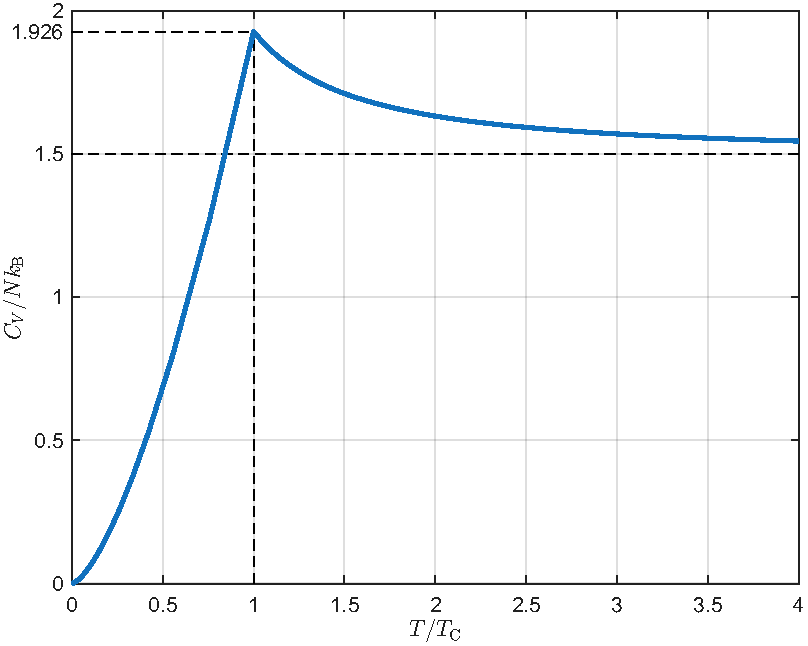
\includegraphics[width=0.7\linewidth]{figures/C_VBoson.pdf}
	\captionof{figure}{理想Bose气体热容$C_V$随温度的变化}
\end{center}

\begin{remark}
	% 由于历史条件,当时还不知道全同多粒子系存在(量子起源的)统计关联:对Bose子是有效吸引;而Fermi子是有效排斥。因此,即使没有动力学相互作用,仍可在一定条件下由于有效相互作用而发生凝聚现象。这是一种纯粹量子起源的相变。
	
	实现Bose-Einstein凝聚极其困难,原则上要使气体冷却至
	$n\lambda_T/g_s\geq\zeta(3/2)\approx 2.612$,
	但大多数情况下,在远高于BEC的$T_\crt$到达以前,已发生液化甚至固化的相变。为了实现原子气体的BEC,必须用极稀薄的气体,且要求
	\begin{center}
		二体弹性碰撞的弛豫时间$\ll$形成分子集团的非弹性碰撞的弛豫时间
	\end{center}
	对于碱金属原子气体,前者$\sim\SI{10}\ms$,而后者有几秒至几分钟。%$\tau_\mathrm{elas}\ll$$\tau_\mathrm{inelas}$
	
	% BEC-BCS Crossover Fermionic condensation.
\end{remark}

% \paragraph{液He}

% $T_\crt=\SI{2.17}\K$,$T<T_\crt$时的液He II具有超流性。

% $T=T_\crt$时,比热趋于无穷,$C_T\vs T$曲线形似$\lambda$,故称$\lambda$相变。

\subsection{光子气体}

光子是一种特殊的Bose子,严格来说,光子没有Bose-Einstein凝聚\footnote{广义上来说,赋予光子以质量是可以发生BEC的。}。讨论黑体辐射,$T,V$给定,满足相对论关系
\begin{align}
	\varepsilon=h\nu=cp.
\end{align}
光子间无相互作用,符合理想气体。%光子自旋$s=1$,简并度$g_s=2$;
光子质量为0,因此$\lambda_T\to\infty$,且光子数不守恒,没有$\alpha$
\[
	a_i=\frac{\omega_i}{\e{\beta\varepsilon_i}-1}.
\]
\begin{theorem}
	{Planck黑体辐射定律}{Planck blackbody radiation}
	能完全吸收电磁波的物体,称为黑体。黑体辐射的能量谱为
	\begin{subequations}
		\begin{align}
			u(\nu)\d\nu&=\frac{8\pi h\nu^3}{c^3}\frac1{\e{\beta h\nu}-1}\d\nu,\\
			u(\lambda)\d\lambda&=\frac{8\pi hc}{\lambda^5}\frac1{\e{\beta hc/\lambda}-1}\d\lambda.
		\end{align}
	\end{subequations}
	\begin{center}
		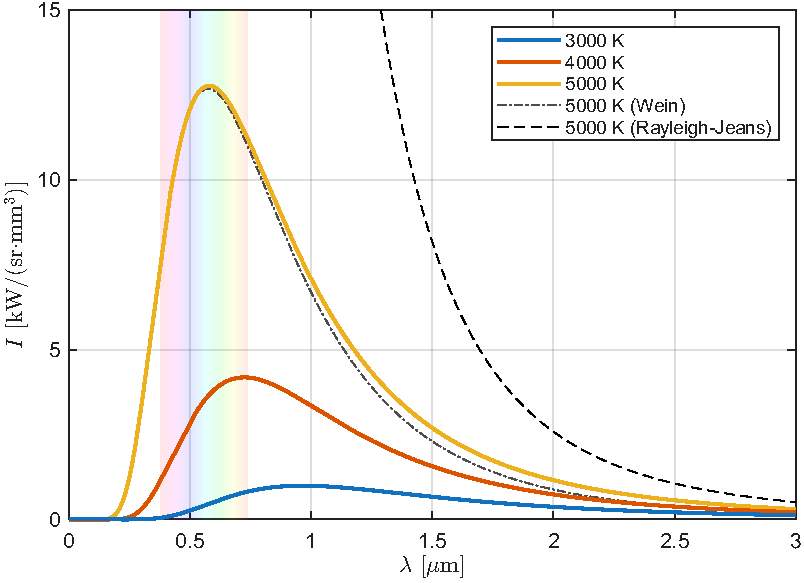
\includegraphics[width=0.8\linewidth]{figures/blackbody.pdf}
		\captionof{figure}{黑体辐射能谱}
		\label{fig:blackbody radiation}
	\end{center}
\end{theorem}

\begin{proof}
	假设$V$很大,能量准连续,$(\nu,\nu+\d\nu)$内的微观状态数
	\[
		g(\varepsilon)\d\varepsilon=\frac{g_sV}{h^3}\frac{4\pi}{c^3}\varepsilon^2\d\varepsilon\implies g(\nu)\d\nu=g(h\nu)h\d\nu=\frac{4\pi g_sV}{c^3}\nu^2\d\nu.
	\]
	其中光子的自旋因子$g_s=2$,
	光子数
	\[
		N(\nu)\d\nu=\frac{g(\nu)\d\nu}{\e{\beta h\nu}-1}.
	\]
	可得能量谱
	\[
		u(\nu)\d\nu=\frac{N(\nu)}Vh\nu\d\nu=\frac{h\nu}V\frac{g(\nu)\d\nu}{\e{\beta h\nu}-1}=\frac{8\pi\nu^2}{c^3}\frac{h\nu}{\e{\beta h\nu}-1}\d\nu.
	\]
	改为波长
	\[
		u_\lambda(\lambda)\d\lambda=u_\nu\biggkh{\frac c\lambda}\frac c{\lambda^2}\d\lambda=\frac{8\pi hc}{\lambda^5}\frac1{\e{\beta hc/\lambda}-1}\d\lambda.
		\qedhere
	\]
\end{proof}

\begin{corollary}
	在低频高温和高频低温极限下,可分别得到经典的\Rayl-Jeans规律和Wein规律
	\[
		u(\nu)\d\nu\simeq
		\begin{cases}
			\frac{8\pi\nu^2}{c^3}\kB T\d\nu,&h\nu\ll\kB T\\[1ex]
			\frac{8\pi h\nu^3}{c^3}\e{-\beta h\nu}\d\nu,&h\nu\gg\kB T
		\end{cases}
	\]
\end{corollary}

\begin{theorem}
	{Stefan-Boltzmann定律}{Stefan-Boltzmann}
	辐射通量密度
	\begin{equation}
		J=\sigma T^4,
	\end{equation}
	其中$\sigma=\SI{5.6704e-8}{\W\per\m\squared\per\K\squared}$称为Stefan-Boltzmann常数。
\end{theorem}

\begin{proof}
	% 由积分恒等式
	% \begin{equation}
	% 	\int\zti\frac{x^{n-1}\d x}{\e x-1}=\Gamma(n)\zeta(n),
	% \end{equation}
	辐射场的总内能密度
	\[
		u=\int\zti u(\nu)\d\nu=\frac{8\pi}{c^3h^3\beta^4}\cdot\Gamma(4)\zeta(4)=\frac{8\pi^5}{15h^3c^3\beta^4}.
	\]
	辐射通量密度
	\[
		J=cu\cdot\frac1{4\pi}\int_{2\pi}\cos\theta\d\Omega
		% =cu\cdot\frac12\int_0^{\pi/2}\cos\theta\sin\theta\d\theta
		=\frac14cu=:\sigma T^4,
		\quad
		\sigma=\frac{2\pi^5\kB^4}{15h^3c^3}.
		\qedhere
	\]
\end{proof}

\begin{remark}
	在国际单位制下,$c,h,\kB$都是精确的,因此$\sigma$也是精确的。
\end{remark}

\begin{theorem}
	{Wein位移定律}{Wein displacement law}
	能谱的最大值点$\lambda_{\mathrm m}$和$\nu_{\mathrm m}$满足
	\begin{subequations}
		\begin{align}
			\frac{\nu_{\mathrm m}}T&=\frac{2.82\kB}{h}=\SI{58.79}{\GHz\per\K},\\
			\lambda_{\mathrm m}T&=\frac{hc}{4.96\kB}=\SI{2.89777}{\mm\K}.		
		\end{align}
	\end{subequations}
\end{theorem}

\begin{proof}
	直接求导$\d u/\nd\nu=0$并令$x:=\beta h\nu$可得
	\[
		x=3(1-\e{-x})\implies x=3+W(-3\e{-3})\approx 2.821439372,
	\]
	其中Lambert $W$函数是$x\e x$的反函数。
	类似地,
	$\d u/\nd\lambda=0$并令$x:=\beta hc/\lambda$可得
	\[
		x=5(1-\e{-x})\implies x=5+W(-5\e{-5})\approx 4.965114231.
		\qedhere
	\]
\end{proof}

\paragraph{热力学函数}

巨配分函数
\begin{equation}
	\ln\Xi=-\int\zti g(\varepsilon)\ln(1-\e{-\beta\varepsilon})\d\varepsilon=\frac{8\pi^5V}{45h^3c^3\beta^3}.
\end{equation}
内能、比热、压强和熵
\begin{subequations}
	\begin{align}
		U&=-\pv{\ln\Xi}\beta=3\frac{\ln\Xi}\beta=\frac{8\pi^5V}{15h^3c^3\beta^4}=4\sigma VT^4,\\
		C_V&=\pu[V]UT=4\frac UT=16\sigma VT^3,\\
		p&=\frac1\beta\pv{\ln\Xi}V=\frac13\frac UV=\frac43\sigma T^4,\\
		S&=\kB(\ln\Xi+0+\beta U)=\frac43\frac UT=\frac{16}3\sigma VT^3,\\
		F&=U-TS=-\frac13U,\\
		G&=F+pV=0\implies\mu=0.
	\end{align}
\end{subequations}
$C_V\propto T^3$随温度上升而增加,$\mu=0$,与光子数不守恒对应。

\subsection{声子气体}

在Einstein模型中,我们将固体晶格振动简谐近似为独立的简谐振子,频率$\nu$,量子数为$n$的振子激发态相当于产生了$n$个能量为$h\nu$的粒子,称为声子(phonon)。
% \[
% 	\varepsilon=\hbar\omega,\quad p=\hbar k;\quad \omega=kv.
% \]
声子气体不可分,符合Bose分布,且声子数不守恒
\[
	a_i=\frac{\omega_i}{\e{\beta h\nu_i}-1}.
\]
声波分为横波(transverse)和纵波(longitudinal),速度分别为$v_\tv$和$v_\lt$;横波有两种振动方式,纵波只有一种。
纵波声子状态数
\[
	g_\lt(\omega)\d\omega=\frac V{h^3}\cdot 4\pi p_\lt^2\d p_\lt=\frac V{2\pi^2v_\lt^3}\omega^2\d\omega.
\]
横波同理,故总状态数
\[
	g(\omega)\d\omega=\frac V{2\pi^2}\kh{2v_\tv^{-3}+v_\lt^{-3}}\omega^2\d\omega=:B\omega^2\d\omega.
\]
其中$B$为与$\omega$无关的比例系数,
Einstein模型定量不符,因为忽略了低频振动,而低温下的热激发主要在低频(长波)部分,当波长$\gg$原子间距时,可看做$0-\omega_\Db$的连续谱,
其中$\omega_\Db$称为Debye频率,
对应的特征温度称为Debye温度:
\[
	\theta_\Db:=\frac{\hbar\omega_\Db}\kB\sim\SI{200}\K.
\]
故
\[
	3N=\int_0^{\omega_\Db}g(\omega)\d\omega=\frac B3\omega_\Db^3\implies B=\frac{9N}{\omega_\Db^3}.
\]
可得
\[
	g(\omega)=\begin{cases}
		9N\omega^2/\omega_\Db^3,&0\leqslant\omega\leqslant\omega_\Db\\
		0,&\omega>\omega_\Db
	\end{cases}
\]
可得内能和比热
\begin{subequations}
	\begin{align}
		U&=U_0+3N\kB T\Debye(y),\\
		C_V&=3N\kB\biggkh{4\Debye(y)-\frac{3y}{\e y-1}}.
	\end{align}
\end{subequations}
其中$y:=\theta_\Db/T=\beta\hbar\omega_\Db$,$\Debye(y)$为Debye函数
\[
	\Debye(y):=\frac 3{y^3}\int_0^{y}\frac{x^3\d x}{\e x-1}.
\]
高温极限$y\ll 1$,
\[
	\Debye(y)=\frac3{y^3}\int_0^y x^3\biggkh{\frac1x-\frac12+\frac x{12}+\bigo(x^3)}\d x=1-\frac38y+\frac{y^2}{20}+\bigo(y^4).
\]
可得 
\begin{subequations}
	\begin{align}
		U&=3N\kB T+U_0-\frac98N\kB\theta_\Db+\frac{3N\kB\theta_\Db^2}{20T}+\bigo\biggkh{\frac1{T^3}},\\
		C_V&=3N\kB-\frac3{20}N\kB\biggkh{\frac{\theta_\Db}T}^2+\bigo\biggkh{\frac1{T^4}}.
	\end{align}
\end{subequations}
低温极限$y\gg 1$,可认为
\[
	\Debye(y)\simeq\frac3{y^3}\int\zti\frac{x^3\d x}{\e x-1}=\frac{\pi^4}{5y^3},
\]
可得
\begin{subequations}
	\begin{align}
		U&\simeq U_0+\frac{3\pi^4}5N\kB\frac{T^4}{\theta_\Db^3},\\
		\label{eq:CV Debye}
		C_V&\simeq\frac{12\pi^4}5N\kB\biggkh{\frac T{\theta_\Db}}^3.
	\end{align}
\end{subequations}
$C_V\propto T^3$,
与实验符合。
\begin{center}
	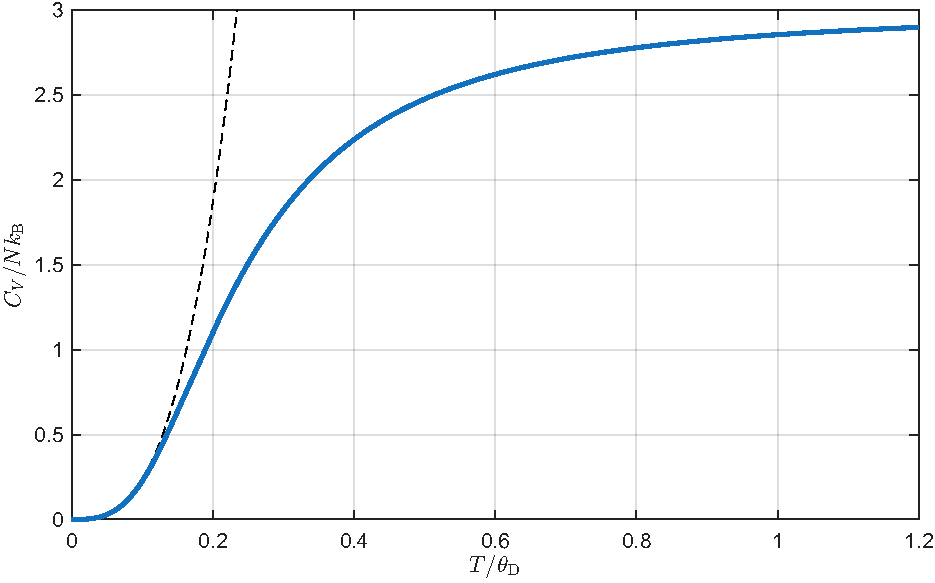
\includegraphics[width=0.8\linewidth]{figures/C_Vphonon.pdf}
	\captionof{figure}{声子气体热容$C_V$随温度的变化}
	\label{fig:CV phonon}
\end{center}

\begin{remark}
	~
\begin{compactenum}
	\item 固体中原子作用强,不能直接用近独立粒子统计。$T$较低时,简谐近似成立——原子集体振动的简正模式。
	相互独立:近独立的理想声子气体。
	\item 声子是准粒子,与振动激发态等效的粒子,有能量、动量等,
	%但不同于电子等,
	只存在于固体中,$\varepsilon$与$p$的关系(色散关系)可不同于普通粒子。
	\item 实际固体比热:金属、自由电子气贡献。

	化合物的分子间振动为声频,适用Debye模型;分子内振动为光频,适用Einstein模型。
\end{compactenum}
\end{remark}

\section{Fermi气体}

讨论简并费米气体的低温性质,
% $n\lambda_T^3\geqslant 1$,相互作用弱。
单个能级$\varepsilon_i$的量子态上的平均粒子数为
\[
	f_i:=\frac{a_i}{\omega_i}=\frac1{\e{\alpha+\beta\varepsilon_i}+1}=\frac1{\e{\beta(\varepsilon_i-\mu)}+1}.
\]

\paragraph{完全Fermi气}

% 讨论$T\to0$时电子的分布,
定义$T=0$时的化学势$\mu(0)=:\varepsilon_\Fm$称为Fermi能量,则
\[
	\lim_{T\to0}f_i=\lim_{T\to0}\frac1{\e{(\varepsilon_i-\mu)/\kB T}+1}=
	\begin{cases}
		1,&\varepsilon_i<\varepsilon_\Fm\\
		0,&\varepsilon_i>\varepsilon_\Fm
	\end{cases}
\]
由Pauli原理,粒子不能都处于$\varepsilon=0$态,但尽可能低,当$\varepsilon<\varepsilon_\Fm$时,各量子态各有一个粒子;而$\varepsilon>\varepsilon_\Fm$时,态无粒子。
Fermi能量可根据粒子数确定:
\begin{equation}
	N=\int_0^{\varepsilon_\Fm}g(\varepsilon)\d\varepsilon=g_s\frac{2\pi V}{h^3}(2m)^{3/2}\cdot\frac23\varepsilon_\Fm^{3/2}
	\implies
	\varepsilon_\Fm=\frac{h^2}{2m}\biggkh{\frac{3n}{4\pi g_s}}^{2/3}.
\end{equation}
进而可得
$T=0$时的零点内能、压强和熵
\begin{subequations}
	\begin{align}
		U_0&=\int_0^{\varepsilon_\Fm}g(\varepsilon)\varepsilon\d\varepsilon=\frac35N\varepsilon_\Fm,\\
		p_0&=-\pv{U_0}V=\frac23\frac{U_0}V=\frac25n\varepsilon_\Fm,\\
		S_0&=\kB\ln\Om[F]=0.
	\end{align}
\end{subequations}

\begin{example}{金属中的电子气}{Electron Gas in Metals}
	电子$m_\elc\sim\SI{e-30}\kg$,数密度$n\sim\SI{e28}{\per\m\cubed}$, % \tothe{3}
	自旋$g_s=2$,故$\varepsilon_\Fm\sim\SI1\eV$,
	\[
		v_\Fm\sim\sqrt{\frac{2\varepsilon_\Fm}m}\sim\SI[per-mode=symbol]{e6}{\m\per\s}
	\]
	压强$p_0\sim\SI{e4}\atm$,这是纯粹的量子效应。
\end{example}

\paragraph{强简并Fermi气}

Fermi温度
\[
	T_\Fm:=\frac{\varepsilon_\Fm}\kB.
\]
对于金属电子气,$T_\Fm\sim\SI{e4}\K$。
低温情形$T\ll T_\Fm$,热运动能量小,粒子分布基本不变,只有$\varepsilon_\Fm\pm\kB T$附近的粒子可能是跳到高能级态上,如\figref{fig:strongly degenerate Fermi gas} 所示。
\begin{center}
	\includegraphics[page=24]{figures/tikz/coordinates.pdf}
	\captionof{figure}{强简并Fermi气粒子分布}
	\label{fig:strongly degenerate Fermi gas}
\end{center}
定性估计比热$C_V$:相对$T=0$时,内能
\[
	U\simeq U_0+N\frac{T}{T_\Fm}\D\varepsilon,
\]
其中$\D\varepsilon\simeq\kB T$,因此
比热
\[
	C_V\simeq 2\kB N\frac{T}{T_\Fm}.
	\tag{approx.}
\]
下面我们给出更定量的结果:
由\secref{sec:weak degeneracy} 的讨论
\[
	C_V=\frac32N\kB\biggfkh{\frac52\frac{\Li_{5/2}(-\e{-\alpha})}{\Li_{3/2}(-\e{-\alpha})}-\frac32\frac{\Li_{3/2}(-\e{-\alpha})}{\Li_{1/2}(-\e{-\alpha})}}.
\]
注意不同于Bose气体,Fermi气体的$\alpha$可正可负。
低温极限$T\ll T_\Fm$,$\alpha\to-\infty$,
对$T/T_\Fm$展开,
\[
	\xi=\frac{n\lambda_T^3}{g_s}=\frac{n}{g_s}\biggkh{\frac{h^2}{2\pi m\kB T}}^{3/2}=\frac4{3\sqrt\pi}\biggkh{\frac{T_\Fm}T}^{3/2}=-\Li_{3/2}(-\e{-\alpha}),
	% =\frac4{3\sqrt\pi}\biggkh{\frac\beta{\beta_\Fm}}^{3/2}.
\]
可得
\begin{subequations}
	\begin{align}
		U&=U_0+\frac{\pi^2}4N\kB T\frac T{T_\Fm}+\bigo(T^3),\\
		\label{eq:CV Fermi}
		C_V&=\frac{\pi^2}2N\kB\cdot\frac T{T_\Fm}+\bigo(T^3).
	\end{align}
\end{subequations}
电子气对金属热容量的贡献首先由Sommerfeld解决。
\begin{center}
	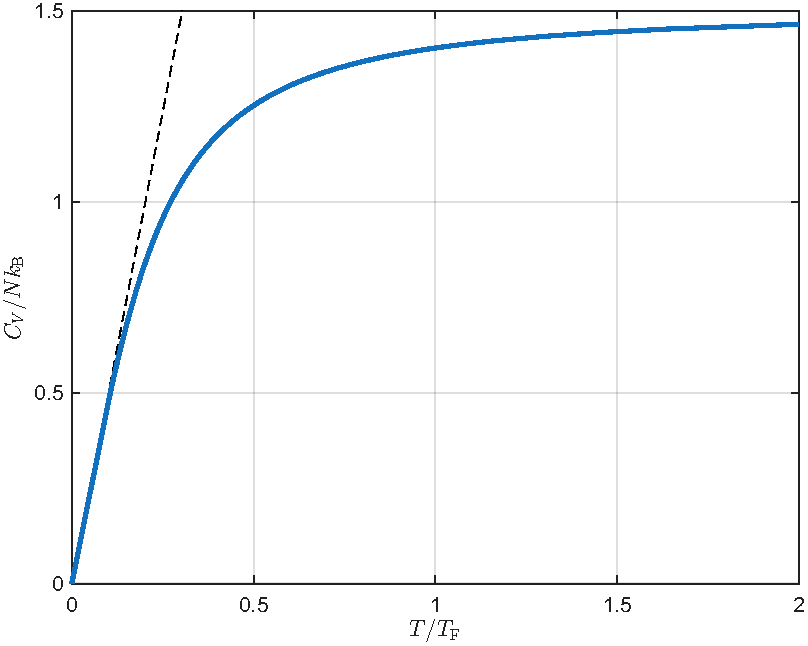
\includegraphics[width=0.8\linewidth]{figures/C_VFermion.pdf}
	\captionof{figure}{Fermi气体比热$C_V$随温度的变化}
\end{center}
因此低温下金属比热的实验值是电子气(Fermi气体)和晶格振动(Debye模型)共同贡献
\[
	C_V\simeq\underset{\text{Fermi}}{c_\elc T}+\underset{\text{Debye}}{c_\vb T^3}.
\]
与实验符合得很好。
\begin{example}{电子比热vs.晶格比热}{}
	低温下,式\eqref{eq:CV Debye}给出晶格比热和式\eqref{eq:CV Fermi}给出电子气比热分别为
	\[
	C_{V,\vb}=N\kB\frac{12\pi^4}5\kh{\frac T{\theta_\Db}}^3,\quad C_{V,\elc}=N\kB\frac{\pi^2}2\frac T{T_\Fm}.
	\]
	对铜,$\theta_\Db\sim\SI{300}\K,\;T_\Fm\sim\SI{8e4}\K$,二者比值
	\[
	\frac{C_{V,\elc}}{C_{V,\vb}}=\frac5{24\pi^2}\frac T{T_\Fm}\kh{\frac{\theta_\Db}T}^3\sim\frac8{T^2}.
	\]
\end{example}